\documentclass[12pt]{report}
\newcommand{\ThesisTitle}{misure di confidenza per algoritmi di stereo vision}
\newcommand{\ThesisAuthor}{Nicola Dal Lago}
\title{\ThesisTitle}
\author{\ThesisAuthor}
\date{}


%%%%%%%%%%%%%%%%%%%%%%%%%% general %%%%%%%%%%%%%%%%%%%%%%%%%%%%%%%%%%%%%%%%%%
\usepackage{a4}
\usepackage{color,colortbl}         
\usepackage[english,italian]{babel}
\usepackage[T1]{fontenc}
\usepackage[utf8]{inputenc}
\usepackage{indentfirst}          
\usepackage{setspace}
\usepackage{float}

%%%%%%%%%%%%%%%%%%%%%% fonts & symbols  %%%%%%%%%%%%%%%%%%%%%%%%%%%%%%%%%%%%%%
\usepackage{amsmath}
\usepackage{amsmath,mathtools}
\usepackage{amsthm}
\usepackage{amsfonts}
\usepackage{amssymb}
\usepackage{fancyvrb}  
\usepackage{xspace}
\usepackage{times}    
\usepackage[overload]{textcase} 

%%%%%%%%%%%%%%%%%%%%%% Floats %%%%%%%%%%%%%%%%%%%%%%%%%%%%%%%%%%%%%%%%
\usepackage{sidecap}
\usepackage{graphicx}
\usepackage{caption}
\usepackage{subfig}
\usepackage{wrapfig}
%\usepackage{subcaption}
\usepackage[algo2e,algochapter,ruled,linesnumbered,vlined]{algorithm2e}

%%%%%%%%%%%%%% page headers and footers %%%%%%%%%%%%%%%%%%%%%%%%%%%%%%
\usepackage{fancyhdr}
\pagestyle{fancy}
\renewcommand{\chaptermark}[1]{
  \markboth{{\bf \chaptername \ \thechapter.} \ #1}{}}
\fancyhead[LE,RO]{\thepage}       
\fancyhead[RE]{\it \small \ThesisTitle }
\fancyhead[LO]{\small \it \leftmark}
\fancyhead[CE,CO]{}                    
\fancyfoot[CE,CO]{}
\fancyfoot[LE,RO]{}
\fancyfoot[RE,LO]{}                    
\renewcommand{\headrulewidth}{1pt}       
\renewcommand{\headheight}{15pt}        
\renewcommand{\footrulewidth}{0pt}      
\addtolength{\headsep}{5mm}

%%%%%%%%%%%%%%%%%%%%% counters %%%%%%%%%%%%%%%%%%%%%%%%%%%%%%%%%%%%%
\setcounter{secnumdepth}{3}
\setcounter{tocdepth}{3}    

%%%%%%%%%%%%%%%% utilities %%%%%%%%%%%%%%%%%%%%%%%%%%%%%%%%%%%%%%%%%%%%
\newcommand{\nullpage}{\newpage\null\thispagestyle{empty}}


\usepackage[
 colorlinks=false,
 a4paper=true,
 linktocpage=true,
 pagebackref=false,
 pageanchor=true,
 hyperindex=true,
 bookmarks=true,
 bookmarksopen=true,
 bookmarksnumbered=true,
 pdffitwindow=true,
 citecolor=blue,
 urlcolor=blue
 ]%
 {hyperref}

\begin{document}

%%----------------------------------- COPERTINA ------------------------------------------------%%

	\setcounter{page}{0}                  %inizia numerazione pagine
	\renewcommand{\thepage}{\roman{page}} %numerazione romana
	\begin{titlepage}
		\begin{center}
			\vbox to0pt{\vbox to\textheight{\vfill 
\includegraphics[width=11.5cm]{./figures/unipd-light} \vfill}\vss}

			\hspace{0.5cm}
			\begin{minipage}{.20\textwidth}
  				
\includegraphics[height=2.5cm]{./figures/unipd-bn}
			\end{minipage}\begin{minipage}{.90\textwidth}
  				\begin{table}[H]
  					\begin{tabular}{l}
  						\scshape{\Large{\bfseries{Università degli Studi di Padova}}} \\
  						\hline \\
  						\scshape{\large{Dipartimento di Ingegneria dell'Informazione}} \\
  					\end{tabular}
  				\end{table}
			\end{minipage}

			\vspace{1.5cm}
			\emph{\Large{Corso~di~Laurea~in~Ingegneria~dell'Informazione}} \\
			
			\vspace{1.5cm}
			\scshape{\Large{\bfseries{\ThesisTitle}}} \\
			\vspace{0.2cm} \linespread{1} \scshape{\large{\bfseries{confidence measures for stereo vision algorithms}}}
		\end{center}

		\vfill
		\begin{normalsize}
			\begin{flushleft}
  
  				\hspace{83pt} \textit{Laureando} \hspace{142pt} \textit{Relatore}\\
  				\vspace{5pt}
  
  				\hspace{62pt} \large{\textbf{Nicola Dal Lago}} \hspace{71pt} \large{\textbf{Prof. Pietro Zanuttigh}}\\
  
  				\vspace{5pt}
  				\hspace{270pt} \textit{Correlatore}\\
  
  				\vspace{5pt}
  				\hspace{247pt} \large{\textbf{Dott. Giulio Marin}}\\
			\end{flushleft}
		\end{normalsize}

		\vfill
		\begin{center}
			\hspace{-0.2cm}
			\line(1, 0){360}

			\textsc{Anno Accademico 2013/2014}
		\end{center}
 	\end{titlepage}


%%------------------------------ ABSTRACT -----------------------------------------%%
	\nullpage                      %pagina bianca

	\chapter*{Abstract}
	\label{sec:Abstract}
	\addcontentsline{toc}{chapter}{Abstract}
	\pagestyle{fancy}
	
	\#TODO: srivere qui l'abstract
	

%%------------------------------ INDICE -------------------------------------------%%
	\nullpage						%pagina bianca			
	\tableofcontents				%indice
	\nullpage						%pagina bianca

	\renewcommand{\thepage}{\arabic{page}} %numerazione normale
	\setcounter{page}{1}                   %inizia numerazione pagine


%%----------------------------- INTRODUZIONE ---------------------------------------%%	
	\chapter{Introduzione}
	\label{sec:introduzione}
	\pagestyle{fancy}
	
		La visione stereo è stata un'area attiva della della ricerca per decenni. Negli ultimi anni, gli algoritmi di stereo vision sono maturati a tal punto da essere applicati in un vasto scenario, dalla automazione industriale, al gaming fino alla guida assistita \cite{mercedes}.
	
		\section{Stereopsi}
		\label{sec:Stereopsi}
			\textit{
			La stereopsi è la capacità percettiva che consente di unire le immagini provenienti dai due occhi, che a causa del loro diverso posizionamento strutturale, presentano uno spostamento laterale. Questa disparità viene sfruttata dal cervello per trarre informazioni sulla profondità e sulla posizione spaziale dell'oggetto mirato. Di conseguenza la stereopsi permette di generare la visione tridimensionale. \footnote{da \url{https://it.wikipedia.org/wiki/Stereopsi}} \newline}
			
			Si possono quindi identificare due problemi: calcolo delle corrispondenze e triangolazione \cite{fusiello}.\newline
			Il primo consiste nell'accoppiare punti delle due immagini, detti punti coniugati, che sono proiezione dello stesso punto nella scena. Il calcolo delle corrispondenze è un problema possibile in quanto le due immagini differiscono di poco, quindi un punto della scena deve apparire simile nei punti coniugati delle due immagini. Basando solo su questo però, sono possibili molti accoppiamenti sbagliati; le due immagini vengono quindi rettificate prima del calcolo delle corrispondenze, in modo che due punti coniugati si trovino sulla stessa retta (detta retta epipolare). Questo si ottiene ruotando le immagini originali attorno ai loro centri ottici finché i piani 
			focali non diventano co-planari (e quindi anche i piani immagine).\newline
			Per triangolazione si intende il calcolo della distanza tra un punto della scena e il piano formato dalle due fotocamere. Nel caso di due fotocamere parallele ed allineate ci si può facilmente ricondurre alla figura \ref{fig:triangolazione}.\newline
			Fissato come riferimento la fotocamera di sinistra si possono scrivere le equazioni di proiezione prospettica:
			
			\begin{equation}
				\begin{dcases}
					\frac{f}{z}=\frac{-u}{x} \\
					\frac{f}{z}=\frac{-u'}{x-b}
				\end{dcases}
				\label{eq:sistema}
			\end{equation}
			
			\begin{SCfigure}[]
				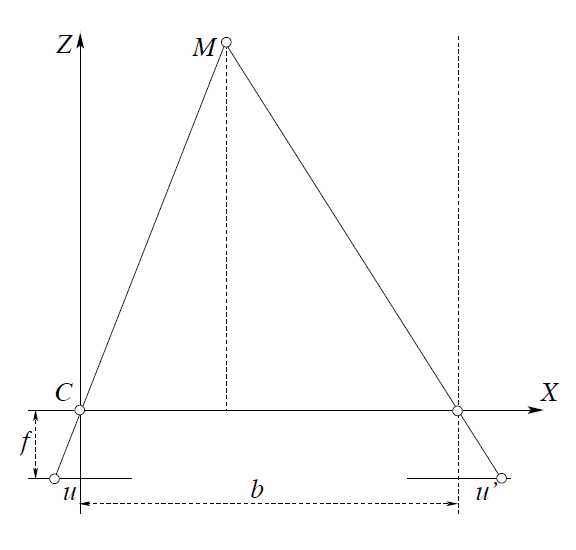
\includegraphics[width=0.6\textwidth]{./figures/Triangolazione_stereoscopica.png}
				\caption{Triangolazione stereoscopica.}
				\label{fig:triangolazione}
			\end{SCfigure}
			
			\noindent e risolvendo si ottiene:

			\begin{equation}
				z=\frac{bf}{u'-u}
				\label{eq:soluzione}
			\end{equation}
			
			\noindent dove $b$ è la distanza tra le due fotocamere, $f$ la focale delle fotocamere e $u'-u$ la distanza fra i due centri ottici.
		
		
		\section{Calcolo delle corrispondenze}
		\label{sec:corrispondenze}
		
			\begin{figure}
				\subfloat[][\emph{Fotocamera di destra}.]
				{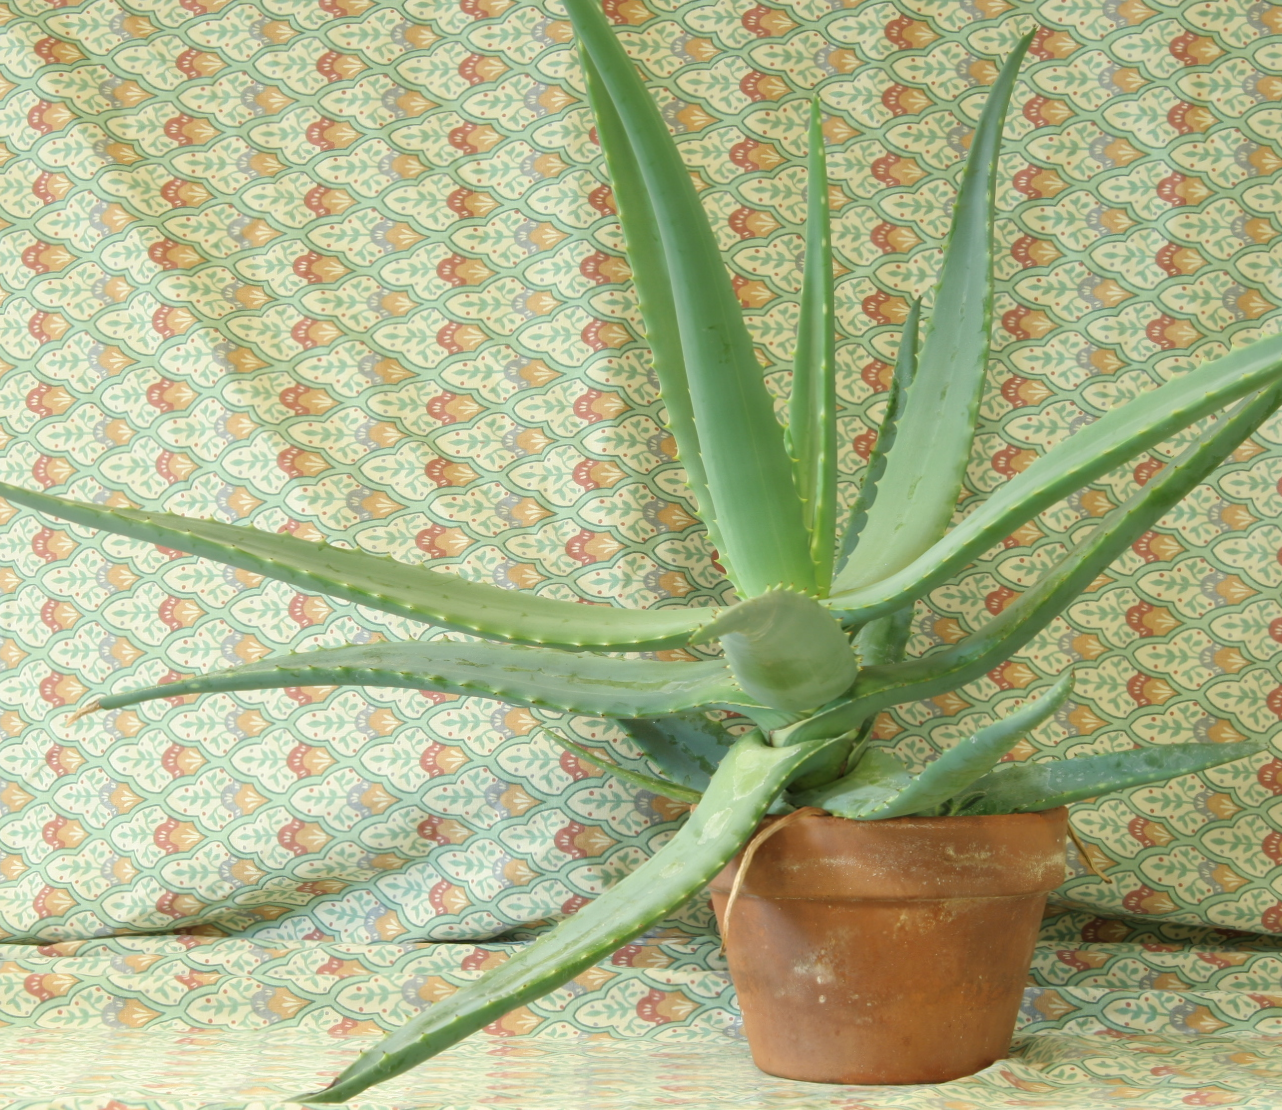
\includegraphics[width=.31\textwidth]{./figures/view1.png}} \quad
				\subfloat[][\emph{Fotocamera di sinistra}.]
				{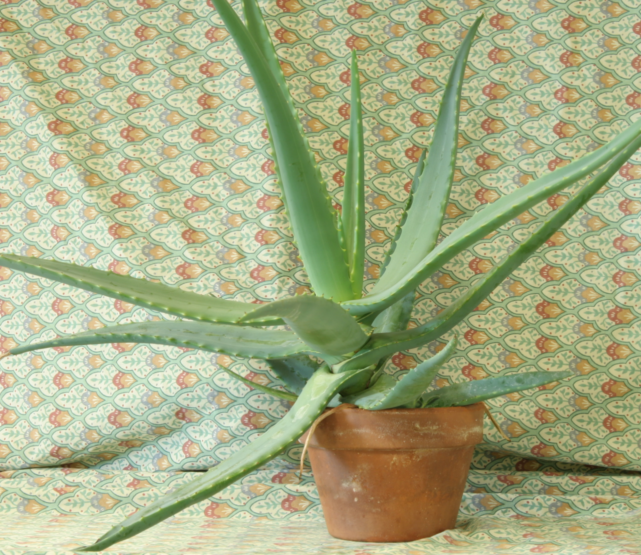
\includegraphics[width=.31\textwidth]{./figures/view5.png}} \quad
				\subfloat[][\emph{Mappa di disparità}.]
				{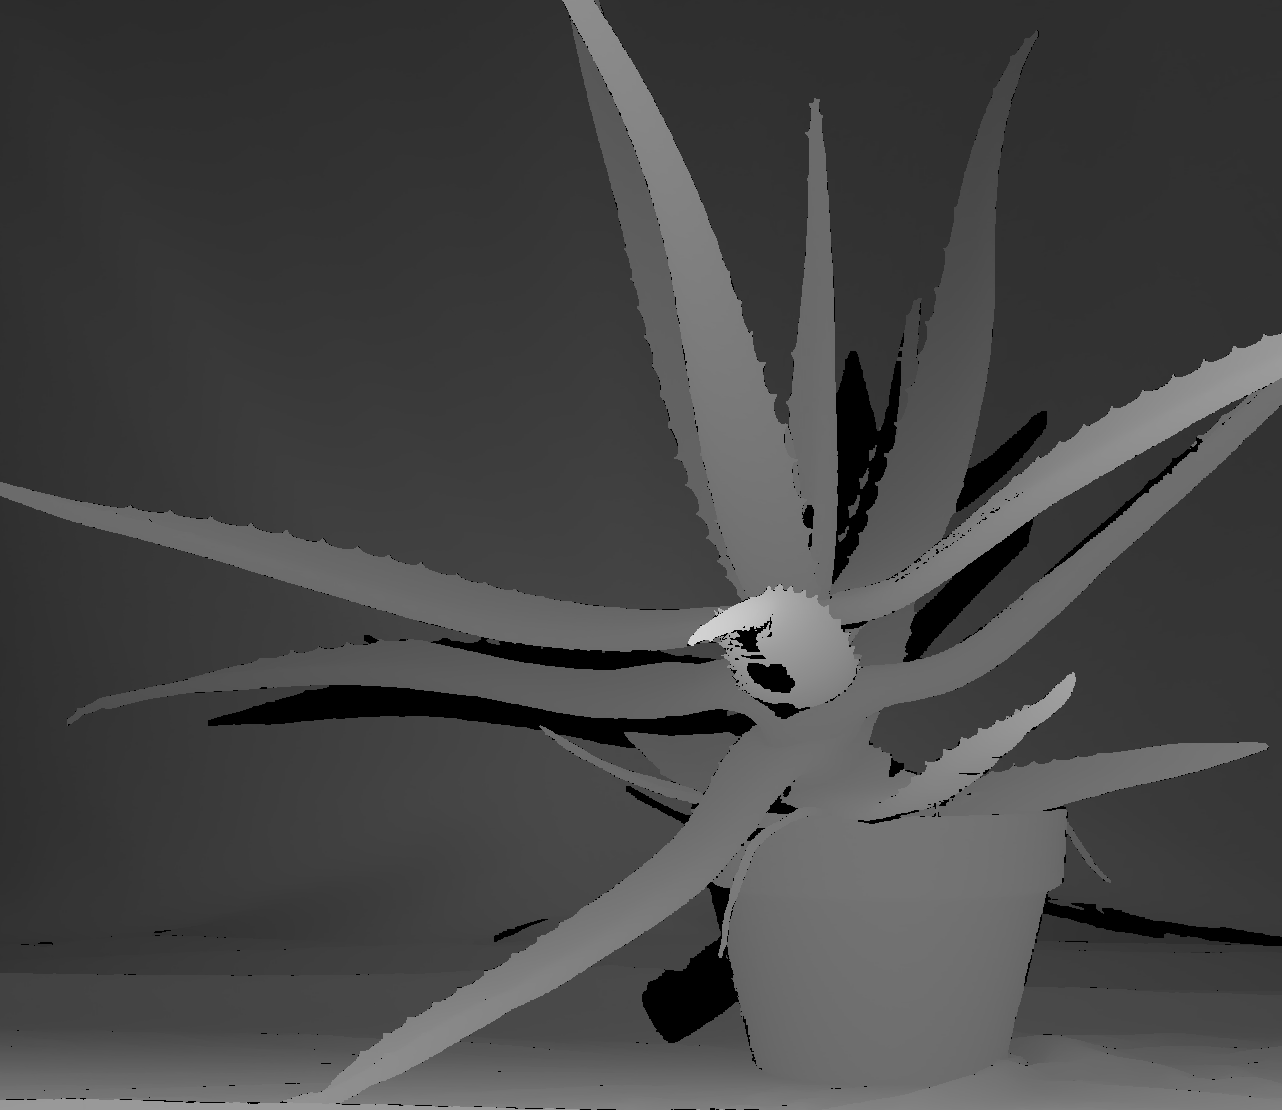
\includegraphics[width=.31\textwidth]{./figures/disp1.png}} 
				\caption{Mappa di disparità con immagine di destra come riferimento, immagine presa da \url{http://vision.middlebury.edu/stereo/data/}}
				\label{fig:disparità}
			\end{figure}
			
			
			
			Il calcolo delle corrispondenze o della disparità è il problema principale della stereo vision. \newline
			La disparità è la differenza tra due punti coniugati, immaginando di sovrapporre le due immagini. Il calcolo delle corrispondenze non è altro che il calcolo della disparità per ogni pixel delle due immagini \cite{fusiello}. Si ottiene quindi una mappa di disparità del tipo di figura \ref{fig:disparità}.\newline
			Gli approcci tipici per il calcolo della disparità sono basati su correlazione \cite{correlation} o semi-global matching (SGM) \cite{SGM}. In questa tesi viene utilizzato un algoritmo SGM, questo tipo di algoritmi usa una regione dell'immagine al posto del singolo pixel per identificare i punti coniugati. Ogni punto viene confrontato con tutti i punti nella retta epipolare, ad ogni pixel viene dato un costo e quindi si forma una cosiddetta funzione di costo.
			

			



%%--------------------------- MISURE DI CONFIDENZA ------------------------------------%%						
	\chapter{Misure di confidenza}
	\label{sec:confidenza}
	\pagestyle{fancy}
	
		Come accennato in \ref{sec:corrispondenze}, ad ogni pixel dell'immagine di riferimento (destra o sinistra), viene assegnata una funzione costo, la quale identifica quanto il pixel è "simile" al suo possibile coniugato.
			
			
		\begin{figure}[<h>]
			\centering
			\subfloat[][\emph{Funzione costo ideale}.]
			{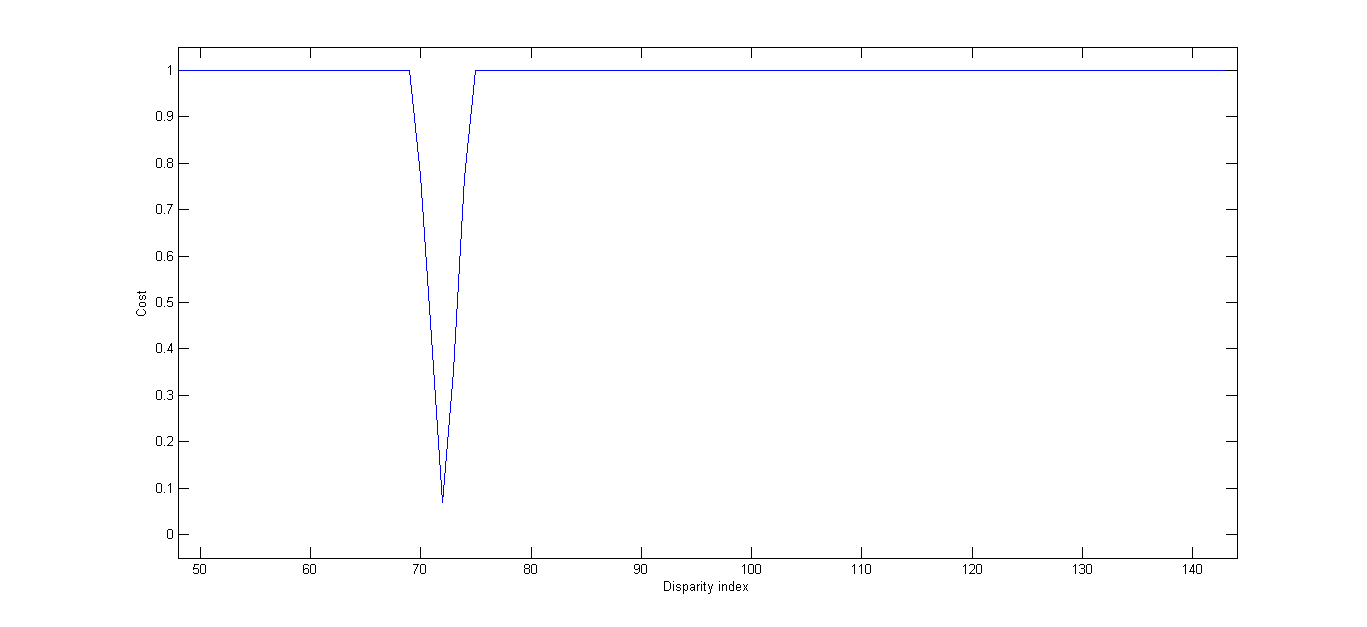
\includegraphics[width=.48\textwidth]{./figures/good_cost.png}} \quad
			\subfloat[][\emph{Funzione costo ambigua}.]
			{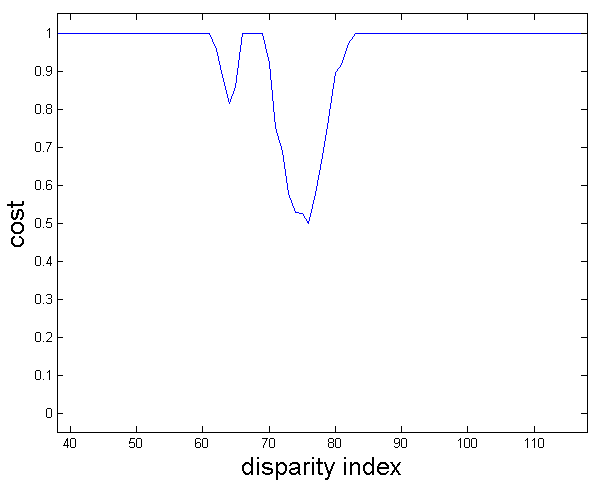
\includegraphics[width=.48\textwidth]{./figures/bad_cost.png}}
			\caption{Due possibili funzioni costo}
			\label{fig:costi}
		\end{figure}	
		
		\noindent Due possibili funzioni costo sono riportate in figura \ref{fig:costi}. E' chiaro che nel primo caso il punto coniugato  è individuato da quell'unico picco; nel secondo caso invece, la funzione è ambigua, in quanto vi sono diversi picchi, e non è quindi più così banale trovare il punto coniugato. Si rende quindi necessario lo studio di varie tecniche per misurare la confidenza di ciascun picco.
		
		
		\section{Implementazione utilizzata}
		\label{sec:implementazione}
		
		Per il calcolo della funzione costo, è stato utilizzato un algoritmo di semi-global matching presente nelle librerie di \textit{OpenCV} \cite{opencv}, scritto nel linguaggio C++. Si ottiene quindi una matrice, in formato \textit{.dat} delle stesse dimensioni delle immagine originali, ma con la funzione costo salvata in ogni casella. Successivamente la matrice viene convertita in un formato \textit{.mat} per renderla più facile da utilizzare con il linguaggio MATLAB. Poi, con uno script MATLAB vengono calcolate le mappe di disparità utilizzando algoritmi diversi. Le immagini utilizzate sono state prese dal dataset Midleburry \cite{dataset_2006_1,dataset_2006_2} disponibili su \url{http://vision.middlebury.edu/stereo/data/}. \newline
		Prima di proseguire, si rende necessario dare alcune definizioni:
		
		\begin{itemize}
		
			\item $c(d)$: il valore del costo assegnato ad una ipotetica mappa di disparità $d$, per un pixel di coordinate $(x,y)$, è denotato con $c(x,y,d)$ o $c(d)$, se le coordinate del pixel non sono ambigue.
			
			\item $c_{1}$: il minimo valore del costo di un pixel è definito con $c_{1}$ e il corrispondente valore di disparità da $d_{1}$; $c_{1}=c(d_{1})=min\{c(d)\}$.
			
			\item $c_{2}$: con $c_{2}$ viene denotato il secondo valore più piccolo in $d_{2}$, mentre con $c_{2m}$ si denota il secondo minimo locale più piccolo.
			
		\end{itemize}
		Seguono quindi tutte le varie tecniche utilizzate, raggruppate secondo l'aspetto del costo che considerano \cite{indoors_outdoors}.
		
		
		
		\section{Matching Cost}
		\label{sec:matching}
		
			Il \textit{Matching Cost} è usato come una misura di confidenza.
		
			\paragraph{Matching Score Metric (MSM)}
			\label{par:matching}
				
				L'\textit{MSM} è la metrica di confidenza più semplice, viene utilizzata come baseline per le prossime metriche.
				
				\begin{equation}
					C_{MSM}=-c_{1}
					\label{eq:MSM}
				\end{equation}
		
		
		
		
		\section{Proprietà locali della curva}
		\label{sec:localProperties}	
			La forma della curva di costo intorno al minimo (la nitidezza o la planarità) è indice di certezza nella partita.
			
			\paragraph{Curvature (CUR)}
			\label{par:curvature}
			
				E' largamente utilizzata nella letteratura \cite{indoors_outdoors}, ed è definita come
				
				\begin{equation}
					C_{CUR}=-2c(d_{1})+c(d_{1}-1)+c(d_{1}+1)
					\label{eq:CUR}
				\end{equation} 
			
				\noindent se $d_{1}-1$ o $d_{1}+1$ sono fuori dal range di disparità, il punto più vicino del minimo viene usato due volte.
			
			
			
		\section{Minimo locale della curva}
		\label{sec:localMinima}	
		
			Si basa sul concetto che la presenza di altri candidati è un'indicazione di incertezza, mentre la loro assenza di certezza.
			
			\paragraph{Peak Ratio Naive (PKRN)} 
			\label{par:PKRN}
		
				A differenza del \textit{Peak Ratio (PKR)}, che calcola il costo con la formula \ref{PKR}
		
				\begin{equation}
					C_{PKR}=\frac{c_{2m}}{c_{1}}
					\label{PKR}
				\end{equation}
			
				\noindent il \textit{PKRN} non richiede che il numeratore sia un minimo locale. Inoltre la formula è leggermente diversa da quella proposta in letteratura \cite{mercedes}
			
				\begin{equation}
					C_{PKRN}=\frac{c_{2} + \epsilon}{c_{1} + \epsilon} - 1
					\label{PKRN}
				\end{equation}
		
				\noindent \textit{PKRN} può essere visto come una combinazione del \textit{PKR} e \textit{CUR}, che assegna bassa confidenza per le corrispondenze con minimi piatti o concorrenti forti.
			
			\paragraph{Nonlinear Margin (NLM)}
			\label{par:NLM}
			
				è definito come
				
				\begin{equation}
					C_{NLM}= e^{ \frac{ c_{2}-c_{1}} {2\sigma_{NLM}^2}}-1
					\label{eq:NLM}
				\end{equation}
				
				\noindent in questa tesi è stato usato un unico valore del parametro $\sigma_{NLM}$, senza cioè andare ad indagare i diversi risultati ottenibili con diverse varianze.
				
		\section{Intera curva}
		\label{sec:entireCost}
		
			Questi metodi convertono la funzione costo in una distribuzione di probabilità sulla disparità.
			
			\paragraph{Maximum Likelihood Metric (MLM)}
			\label{par:MLM}
			
				Insieme a \textit{PKRN} è una delle metriche più promettenti. Entrambe hanno ottenuto risultati sopra la media sia su immagini indoor che outdoor \cite{indoors_outdoors}.
				La \textit{Maximum Likelihood Metric} è definita come
				
				\begin{equation}
					C_{MLM}= \frac{e^\frac{-c_{1}}{2\sigma_{MLM}^2}}{\sum_{d} e^\frac{c_{i}}{2\sigma_{MLM}^2}}
					\label{eq:MLM}
				\end{equation}  	
			
				\noindent In questo caso $\sigma_{MLM}$ rappresenta l'incertezza della disparità, ed è stata scelta alta in modo conservativo (ad esempio 8), anche per avere una distribuzione più uniforme.
		
				















%%---------------------------- BIBLIOGRAFIA ----------------------------------------%%
	\begin{thebibliography}{1}
		
		\bibitem{fusiello}
		A. Fusiello,
		\emph{Visione Computazionale, appunti delle lezioni},
		\url{http://profs.sci.univr.it/~fusiello},
		2008.

		\bibitem{mercedes}
		D. Pfeiffer, S. Gehrig, N. Schneider,
		\emph{Exploiting the Power of Stereo Confidences},
		IEEE Conference on Computer Vision and Pattern Recognition, 2013.
	
		\bibitem{correlation}
		D. Scharstein, R. Szeliski, 
		\emph{A taxonomy and evaluation of
		dense two-frame stereo correspondence algorithms}, 
		IJCV,47(1-3):7–42, 2002.
		
		\bibitem{SGM}
		H. Hirschmüller, 
		\emph{Accurate and efficient stereo processing
		by semi-global matching and mutual information}, 
		IEEE CVPR, pages 807–814, San Diego, USA, June 2005.
		
		\bibitem{mordohai_pami}
		X. Hu, P. Mordohai,
		\emph{A Quantitative Evaluation of Confidence Measures for Stereo Vision},
		IEEE Transactions on Pattern Analysis and Machine Intelligence, 2012.
		
		\bibitem{indoors_outdoors}
		X. Hu, P. Mordohai,
		\emph{Evaluation of Stereo Confidence Indoors and Outdoors},
		IEEE Conference on Computer Vision and Pattern Recognition (CVPR), San Francisco, USA, June 2010.
		
		\bibitem{dataset_2006_1}
		D. Scharstein, C. Pal,
		\emph{Learning conditional random fields for stereo},
		IEEE Computer Society Conference on Computer Vision and Pattern Recognition (CVPR 2007), Minneapolis, MN, June 2007.
		
		\bibitem{dataset_2006_2}
		H. Hirschmüller, D. Scharstein,
		\emph{Evaluation of cost functions for stereo matching},
		IEEE Computer Society Conference on Computer Vision and Pattern Recognition (CVPR 2007), Minneapolis, MN, June 2007.
		
		\bibitem{opencv}
		\emph{OpenCV library 2.4.9},
		\url{http://opencv.org/}.
		
		
		
	\end{thebibliography}	
	




\end{document}